% \newpage
\section{\textbf{Data:} data augmentation is essential in maintaining plasticity}
\label{Sec: Data}

In this section, we conduct a factorial analysis of DA and Reset, illustrating that DA effectively maintains plasticity.
Furthermore, in comparison with other architectural and optimization interventions, we highlight DA's pivotal role as a data-centric method in addressing VRL's plasticity loss.

% \vspace{-\baselineskip}
\textbf{A Factorial Examination of DA and Reset.}~~
DA has become an indispensable component in achieving sample-efficient VRL applications~\citep{drq, RAD, DrQ-v2, ma2022comprehensive}.
As illustrated by the blue and orange dashed lines in Figure~\ref{Fig:Reset}, employing a simple DA approach to the input observations can lead to significant performance improvements in previously unsuccessful algorithms.
However, the mechanisms driving DA's notable effectiveness remain largely unclear~\citep{ma2023learning}.
On the other hand, recent studies have increasingly recognized that plasticity loss during training significantly hampers sample efficiency~\citep{primacy_bias, dormant_neuron, understanding_plasticity}.
This naturally raises the question: \textit{does the remarkable efficacy of DA stem from its capacity to maintain plasticity?}
To address this query, we undertake a factorial examination of DA and Reset.
Given that Reset is well-recognized for its capability to mitigate the detrimental effects of plasticity loss on training, it can not only act as a diagnostic tool to assess the extent of plasticity loss in the presence or absence of DA, but also provide a benchmark to determine the DA's effectiveness in preserving plasticity.

\begin{figure}[ht]
  \centering
  \vspace{-1\baselineskip}
  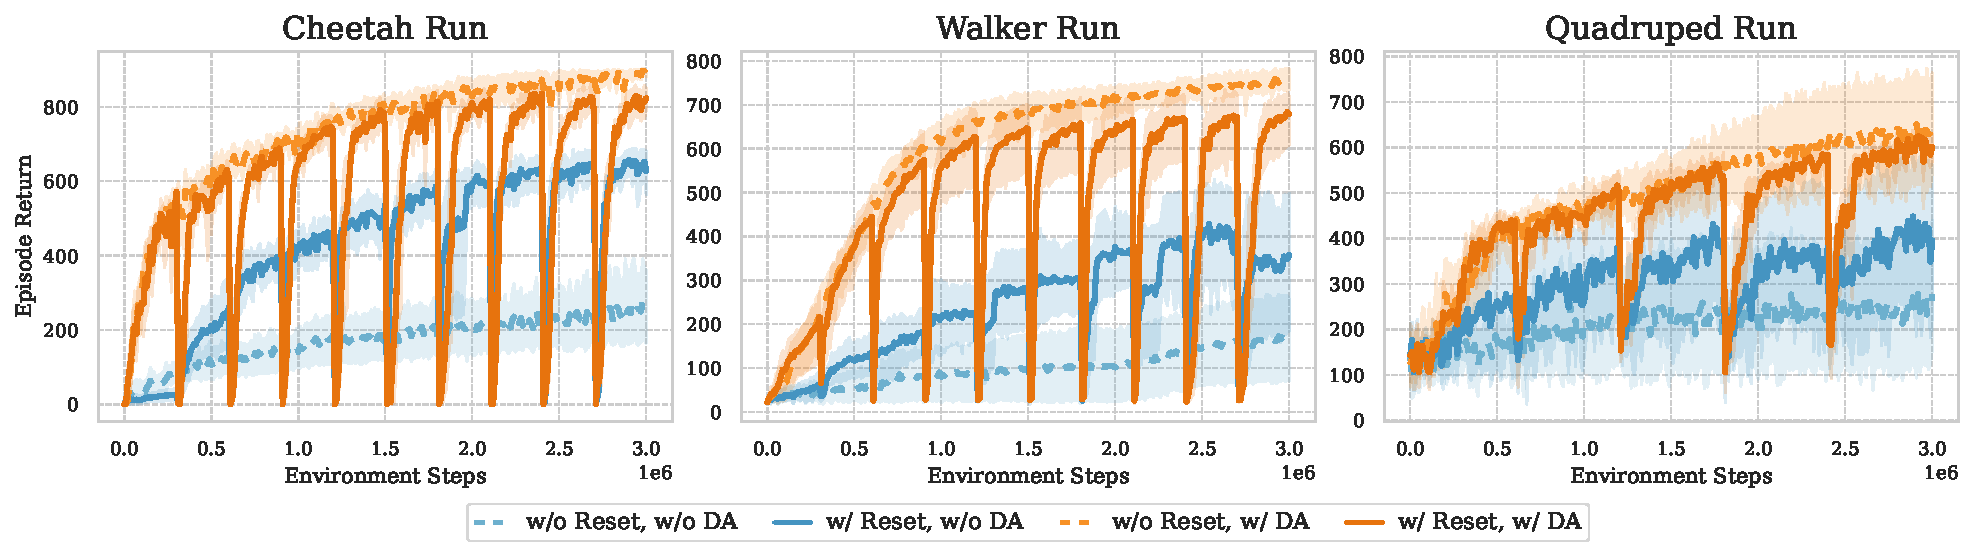
\includegraphics[width=\textwidth]{Figures/1Data/reset_DA_Run.pdf}
  \vspace{-2\baselineskip}
  \caption{Training curves across four combinations: incorporating or excluding Reset and DA.
  We adopt DrQ-v2~\citep{DrQ-v2} as our baseline algorithm and follow the Reset settings from~\cite{primacy_bias}.
  Mean and std are estimated over 5 runs.
  Note that re-initializing 10 times in the Quadruped Run task resulted in poor performance, prompting us to adjust the reset times to 5.
  For ablation studies on reset times and results in other tasks, please refer to \Appendix~\ref{Appendix: Reset}.
  }
  % \vspace{-0.5\baselineskip}
  \label{Fig:Reset}
\end{figure}

\vspace{-0.5\baselineskip}
The results presented in Figure~\ref{Fig:Reset} highlight three distinct phenomena:
\textcolor{mydarkgreen}{$\bullet$} In the absence of DA, the implementation of Reset consistently yields marked enhancements. This underscores the evident plasticity loss when training is conducted devoid of DA.
\textcolor{mydarkgreen}{$\bullet$} With the integration of DA, the introduction of Reset leads to only slight improvements, or occasionally, a decrease. This indicates that applying DA alone can sufficiently preserve the agent's plasticity, leaving little to no room for significant improvement.
\textcolor{mydarkgreen}{$\bullet$} Comparatively, the performance of Reset without DA lags behind that achieved employing DA alone, underscoring the potent effectiveness of DA in preserving plasticity.

% In addition, \Appendix~\ref{Appendix: Heavy Priming}
\begin{wrapfigure}[12]{r}{0.41\textwidth}
  \vspace{-1.2\baselineskip}  
  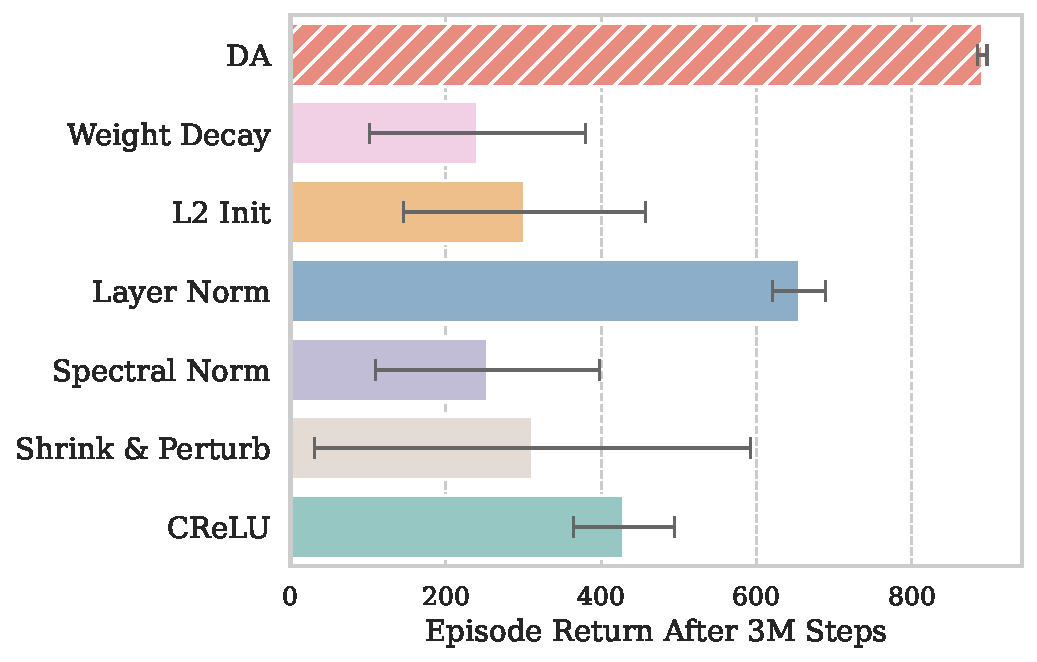
\includegraphics[width=0.41\textwidth]{Figures/1Data/reg_CR.pdf}
  \vspace{-2.1\baselineskip}
  \caption{Performance of various interventions in Cheetah Run across 5 seeds.}
  \label{fig:reg}
\end{wrapfigure}
\textbf{Comparing DA with Other Interventions.}
We assess the influence of various architectural and optimization interventions on DMC using the DrQ-v2 framework. Specifically, we implement the following techniques: 
\textcolor{mydarkgreen}{$\bullet$}~\textit{\textbf{Weight Decay}}, where we set the L2 coefficient to $10^{-5}$.
\textcolor{mydarkgreen}{$\bullet$} \textit{\textbf{L2 Init}}~\citep{Regenerative_Regularization}: This technique integrates L2 regularization aimed at the initial parameters into the loss function. Specifically, we apply it to the critic loss with a coefficient set to $10^{-2}$.
\textcolor{mydarkgreen}{$\bullet$} \textbf{\textit{Layer Normalization}}\citep{layer_norm} after each convolutional and linear layer.
\textcolor{mydarkgreen}{$\bullet$} \textbf{\textit{Spectral Normalization}}\citep{miyato2018spectral} after the initial linear layer for both the actor and critic networks.
\textcolor{mydarkgreen}{$\bullet$} \textbf{\textit{Shrink and Perturb}}\citep{shrink_and_perturb}: This involves multiplying the critic network weights by a small scalar and adding a perturbation equivalent to the weights of a randomly initialized network.
\textcolor{mydarkgreen}{$\bullet$} Adoption of \textbf{\textit{CReLU}}~\citep{shang2016understanding} as an alternative to ReLU in the critic network.
We present the final performance of different interventions in Figure~\ref{fig:reg}, which indicates that DA is the most effective method.
For further comparison of interventions, see \Appendix~\ref{Appendix: Further_Comparisons}.

% \begin{table}[htbp]
% \centering
% % \vspace{-0.5\baselineskip}
% \caption{Regularization}
% \label{DM Control Results}
% \renewcommand{\arraystretch}{1.15}
% % \begin{small}
% % \setlength{\tabcolsep}{2pt}
% \resizebox{\linewidth}{!}{
% \begin{tabular}{lccccccc}
% \toprule
% Tasks & DA & Weight Decay  & L2 Init & Layer Norm & Spectral Norm & Shrink $\&$ Perturb & CReLU \\
% \midrule
% Cheetah Run & $891 \pm 6$ & $0.7 \pm 0.2$ & $301 \pm 156$ & $655 \pm 34$ & $254 \pm 144$ & $312 \pm 281$ & $429\pm 65$ \\
% \bottomrule
% \end{tabular}
% }
% \end{table}

% \paragraph{The effectiveness of DA diminishes with increasing Replay Ratio (RR).}